% Extracción de caracteristicas clásicas
\section{Extracción y coincidencia de características}
% https://medium.com/@deepanshut041/introduction-to-feature-detection-and-matching-65e27179885d
% https://medium.com/@deepanshut041/introduction-to-sift-scale-invariant-feature-transform-65d7f3a72d40

El objetivo de extracción y coincidencia es el de descubrir una o varias características en dos instancias que permitan reconocer e identificar de forma inequívoca, existe multitud de métodos en \acrfull{CV} para detectar puntos de interés. En esta sección discutiremos los métodos y herramientas que podemos emplear usando de ejemplo las librerías de OpenCV y Scikit-Image.

Existen cientos de aplicaciones en la sociedad y en el mundo industrial, médico, automovilístico, militar, etc. Se incluyen tareas de reconstrucción de imágenes, imágenes 3D, mapeo, estabilización de vídeo, etc. 

Uno de los grandes retos es automatizar robots para que reconozcan y puedan interactuar con el entorno. Para ello se debe reconstruir en 3D el entorno para determinar distancias entre objetos, este es uno de los problemas más difíciles, ya que se deben tener en cuenta puntos de vista, iluminación, oclusión, características de los sensores, etc. Por esta razón, estos métodos deben ser robustos ante problemas de oclusión, rotación, escala, iluminación, deformación, etc. \cite{A-survey-of-feature-matching-methods}

En estudios similares se hace mención de los distintos vectores de ataque que pueden sufrir estos sistemas biométricos, en la denominada ``cadena de suministro''. \cite{Debiasi20b} como podemos observar en la Figura \ref{fig:attack-vectors}.

\begin{figure}[H]
    \centering
    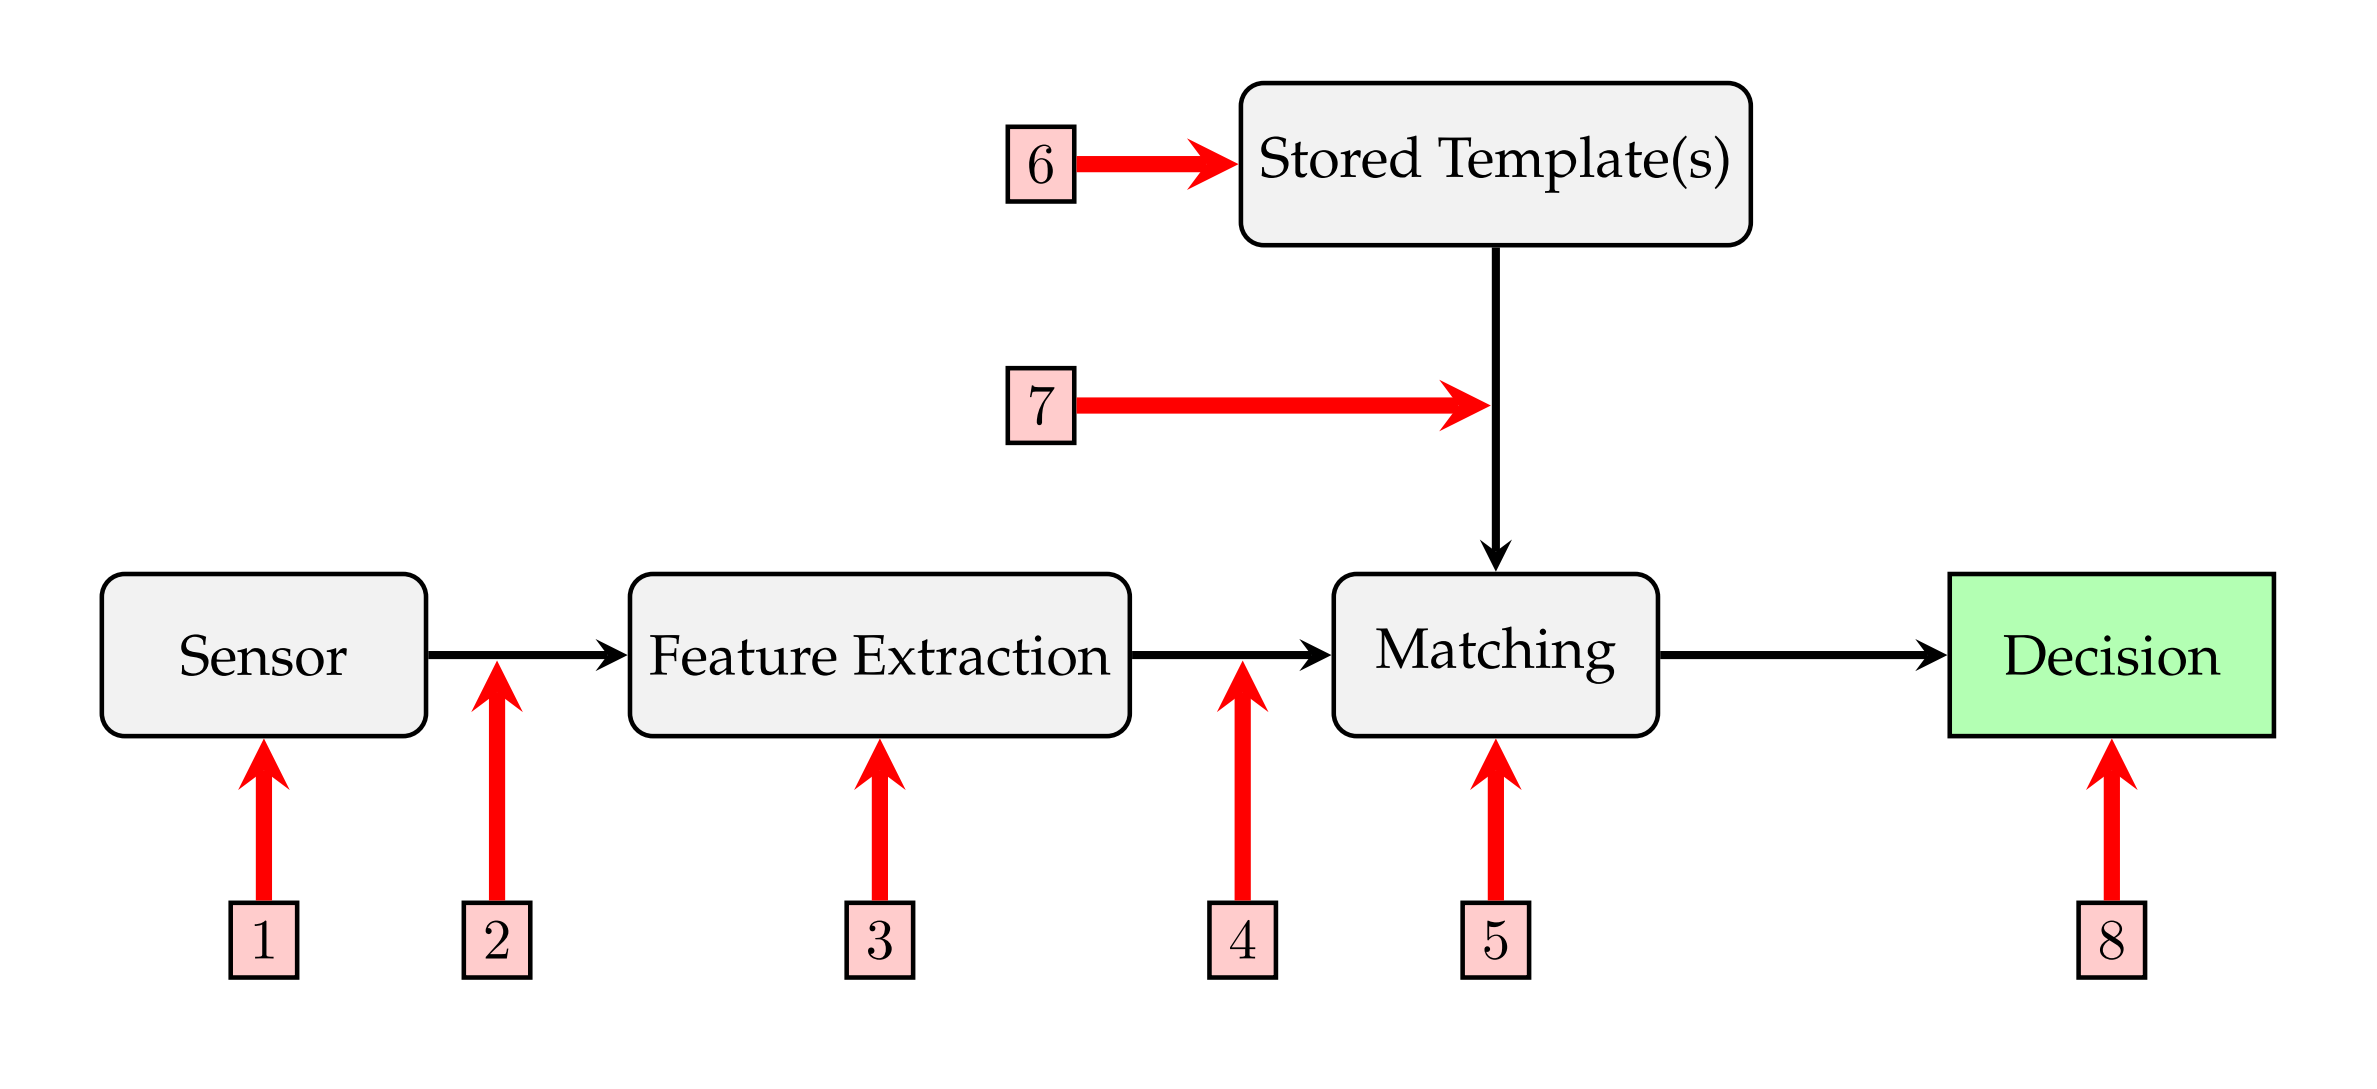
\includegraphics[width=0.8\linewidth]{figures/chapter04/Attack vectors in a generic biometric system.png}
    \caption{Attack vectors in a generic biometric system\newline{}Fuente: Exploiting Image Sensor Data in Biometric Systems and Mobile Applications \cite{Debiasi20b}}
    \label{fig:attack-vectors}
\end{figure}

Actualmente, se clasifican los algoritmos en métodos basados en \textbf{regiones} o métodos basados en \textbf{características}. En los métodos por regiones usan la comparación directa, estos emplean una ventana deslizante que comparará ambas regiones. Los métodos basados en características ofrecen más flexibilidad y estabilidad, estos métodos busca detectar estructuras (esquinas, bordes, formas), con el objetivo de generar descriptores robustos. Se debe tomar las muestras validando de que sean útiles, que no haya un sobre muestreo. Estos métodos dan buenos resultados, pero a costa de un coste computacional muy elevado cuando la resolución de imágenes o vídeos aumenta.

La extracción de características debe ser robusta para su posterior comparación, los métodos por \gls{ANN} usan capas convolucionales, estas capas generarán descriptores basados en las coordenadas de las características y sus relaciones de vecindad. También existen los extractores \textit{end-to-end} que permiten generar los descriptores directamente desde imágenes.

\begin{figure}[H]
    \centering
    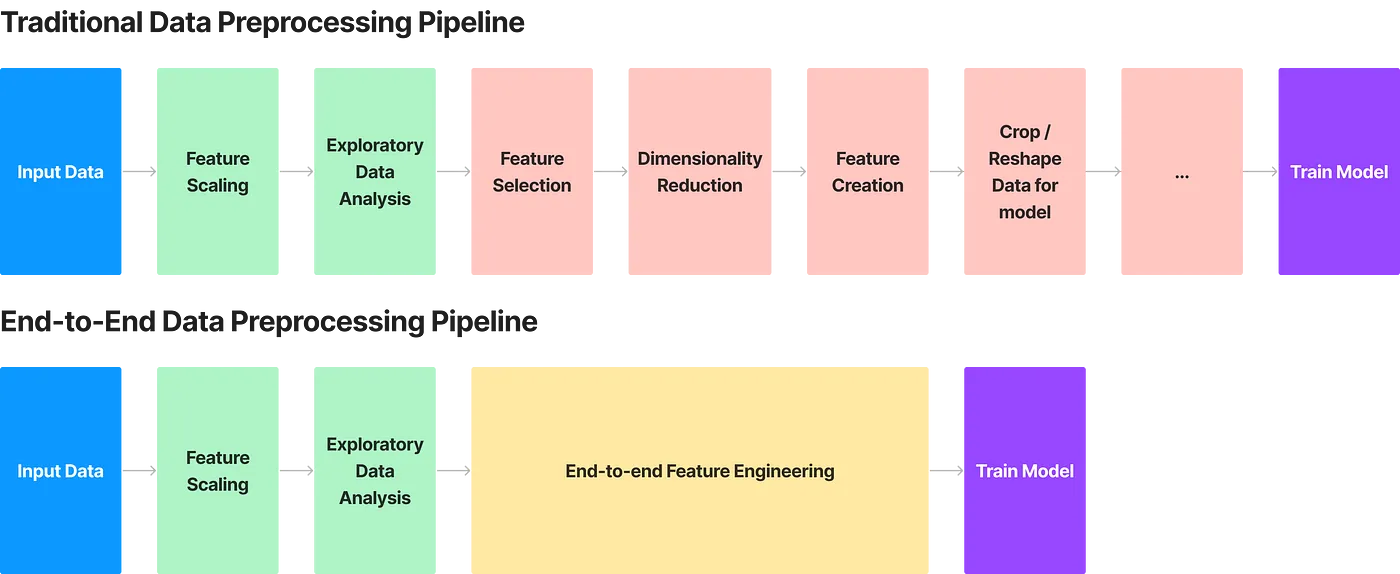
\includegraphics[width=0.5\linewidth]{figures/chapter02/end-to-end.png}
    \caption{End to end feature engineering methods \\Fuente: \href{https://ryendu.medium.com/end-to-end-transformational-feature-engineering-with-cnns-52a5125a10}{End-to-end transformational Feature Engineering with CNNs}}
    \label{fig:end-to-end-cnn}
\end{figure}

\begin{figure}[H]
    \centering
    % 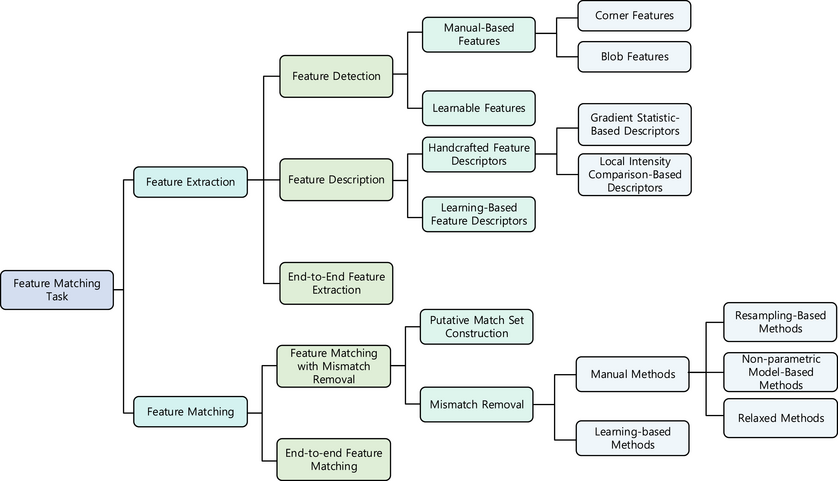
\includegraphics[width=0.5\linewidth]{figures/chapter04/Classification-of-feature-matching-methods.png}
    \centerline{\includesvg[width=1\linewidth]{figures/chapter04/Classification-of-feature-matching-methods.drawio.svg}}
    \caption{Clasificación de métodos de extracción y coincidencia de características. \\Fuente: A survey of feature matching methods \cite{A-survey-of-feature-matching-methods}}
    \label{fig:classification-of-feature-matching-methods}
\end{figure}

Como podemos ver en la Figura \ref{fig:classification-of-feature-matching-methods} existen una gran variedad de métodos y para las distintas tareas dentro de la extracción y coincidencia en \acrfull{CV}, a continuación se listan los algoritmos clásicos más relevantes en la literatura actual. Posteriormente, se identificarán algunos de los métodos de redes neuronales más relevantes en la literatura que permiten también extraer y comparar puntos de interés.

\footnotetext[1]{OpenCV Python cuenta con una implementación experimental.}
\footnotetext[2]{Algoritmo patentado hasta el año 2020}
\footnotetext[3]{Algoritmo patentado hasta el año 2028}


Algunas de las herramientas que permite usar estos algoritmos y métodos son las librerías de \texttt{OpenCV} y \texttt{scikit-image}, estas librerías no implementa todos los métodos que requerimos, pero sí una gran cantidad de ellos.

\begin{figure}[H]
    \centering
    \begin{subfigure}{.25\linewidth}
        \centerline{\includesvg[width=\linewidth]{figures/assets/OpenCV.svg}}
        \caption{Librería OpenCV}
        \label{subfig:opencv}
    \end{subfigure} 
    \hspace{0.10\textwidth} % Espacio horizontal
    \begin{subfigure}{.25\linewidth}
        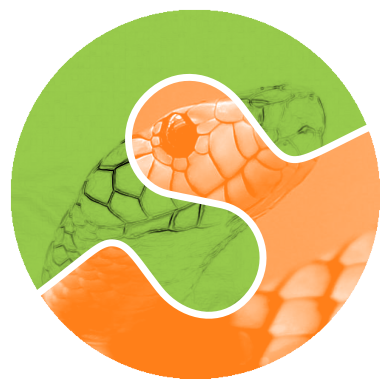
\includegraphics[width=\linewidth]{figures/assets/scikit-image.png}
        \caption{Librería scikit-image}
        \label{subfig:scikit-image}
    \end{subfigure}

    \caption{Librerías para el tratamiento de imágenes}
    \label{fig:libs-images}
\end{figure}


% Distancia Euclidiana: Para descriptores flotantes (SIFT, SURF, etc.).
% Distancia de Hamming: Para descriptores binarios (ORB, BRIEF, BRISK).

% https://riunet.upv.es/bitstream/handle/10251/123298/Agust%C3%AD%20-%20Introducci%C3%B3n%20a%20la%20detecci%C3%B3n%20de%20puntos%20caracter%C3%ADsticos%20con%20OpenCV.pdf?sequence=1
% EL SDK de OpenCV ofrece varios algoritmos para la detección de puntos característicos [7] como AGAST, GFTTDetector, FastFEatureDetector, ORB, AKAZE, BRISK, KAZE o MSER. También existen otros que OpenCV los divide en dos grupos un tanto especiales: experimentales (BoostDesc, BRIEF, DAISY, FREAK, LATCH, LUCID, MSDDetector, PCTSignaturesSQFD, StarDetector o VGG) y extra (compuesto por SIFT, SURF y una versión de SURF optimizada para CUDA,

% Alternativas a SIFT o SURF pueden ser BRISK o FREAK

Explicaremos algunos de los métodos más relevantes y usados en \gls{CV} para la detección de puntos de referencia y sus descriptores. Estos métodos permiten identificar de forma eficiente distintas huellas o identificadores biométricos.

\subsection{Algoritmos de detección de puntos de interés}

\begin{itemize}
    \item \textbf{Bordes}:      % (Operador Roberts cross (1965) \cite{roberts1965machine,angenent2006mathematical}, Robinson (1977) \cite{robinson1977edge}, Canny (1986) \cite{canny1986computational}, Deriche (1987) \cite{deriche1987using}, Differential (1998) \cite{lindeberg1998edge}, STAR Detector (2008) \cite{agrawal2008censure}, Operador Prewitt (2013) \cite{dim2013alternative}, Operador Sobel (2014) \cite{sobelIrwin2014})
    \begin{itemize}
        \item Operador Roberts cross (1965) \cite{roberts1965machine,angenent2006mathematical}
        \item Robinson (1977) \cite{robinson1977edge}
        \item Canny (1986) \cite{canny1986computational}
        \item Deriche (1987) \cite{deriche1987using}
        \item Differential (1998) \cite{lindeberg1998edge}
        \item STAR Detector (2008) \cite{agrawal2008censure}
        \item Operador Prewitt (2013) \cite{dim2013alternative}
        \item Operador Sobel (2014) \cite{sobelIrwin2014}
    \end{itemize}

    \item \textbf{Esquinas}:    % (Harris operator (1988) \cite{Harris88alvey}, Shi-Tomasi (1994) \cite{Shi-and-Tomasi--good-features-to-track}, FAST (1994) \cite{rosten2005fusing,rosten2006machine})
    \begin{itemize}
        \item Harris operator (1988) \cite{Harris88alvey}
        \item Shi-Tomasi (1994) \cite{Shi-and-Tomasi--good-features-to-track}
        \item FAST (1994) \cite{rosten2005fusing,rosten2006machine}
    \end{itemize}
    
    \item \textbf{Blobs}:       % (SIFT\footnotemark[2] (1999) \cite{sift}, AKAZE (2011) \cite{akaze-alcantarilla2011fast})
    \begin{itemize}
        \item SIFT\footnotemark[2] (1999) \cite{sift}
        \item AKAZE (2011) \cite{akaze-alcantarilla2011fast}
    \end{itemize}
    
    \item \textbf{Crestas}:     % (Hough transform (1972) \cite{duda1972use})
    \begin{itemize}
        \item Hough transform (1972) \cite{duda1972use}
    \end{itemize}

    \item \textbf{Regiones}:    % (MSER (2006) \cite{donoser2006efficient})
    \begin{itemize}
        \item MSER (2006) \cite{donoser2006efficient}
    \end{itemize}
\end{itemize}


\subsection{Algoritmos de cálculo de descriptores de puntos de interés}
\begin{itemize}
    \item \textbf{Orientación de gradientes}: 
    \begin{itemize}
        \item SIFT\footnotemark[2] (1999) \cite{sift}
        \item HOG (2005) \cite{dalal2005histograms}
        \item GLOH (2005) \cite{mikolajczyk2005performance}
        \item SURF\footnotemark[3] (2006) \cite{bay2006surf,BAY2008346}
        \item CSIFT (2006) \cite{abdel2006csift}
        \item DAISY\footnotemark[1] (2009) \cite{tola2009daisy}
        \item RootSIFT (2012) \cite{arandjelovic2012three}
    \end{itemize}
    
    \item \textbf{Binarios}: 
    \begin{itemize}
        \item BRIEF\footnotemark[1] (2010) \cite{calonder2010brief}
        \item AKAZE (2011) \cite{akaze-alcantarilla2011fast}
        \item BRISK (2011) \cite{leutenegger2011brisk}
        \item ORB (2011) \cite{rublee2011orb}
        \item LATCH (2016) \cite{Riggan20162016IW}
    \end{itemize}
\end{itemize}


\subsection{Algoritmos de búsqueda de descriptores}
\begin{itemize}
    \item \textbf{Búsqueda lineal}: 
    \begin{itemize}
        \item Brute-Force Matcher \cite{bf-and-flann-matcher}
    \end{itemize}
    
    \item \textbf{Búsqueda aproximada}: 
    \begin{itemize}
        \item FLANN (2012) \cite{bf-and-flann-matcher,10.5555/2354409.2355123}
    \end{itemize}
\end{itemize}

En la literatura se mencionan principalmente dos métodos de búsqueda de descriptores, método por fuerza bruta o búsqueda aproximada (FLANN \cite{bf-and-flann-matcher,10.5555/2354409.2355123}).

Estos métodos presentan ventajas y desventajas, la principal ventaja es que son sencillos y muy eficientes, la principal desventaja el coste computacional cuando la extracción ha dado un gran número de puntos de interés. Actualmente, ya existen métodos que solucionan el problema de alta densidad en la coincidencia de descriptores, como es el caso de \acrshort{FDD} \cite{FDD-pan2024fixedlengthdensedescriptorefficient}.

\subsection{Redes neuronales para la detección y coincidencia}
A continuación se explican otros métodos que son relevantes, ya que usan redes neuronales y métodos de inteligencia artificial para extraer y comprobar la coincidencia de instancias biométricas.

Estos son los métodos \textit{end-to-end} mencionados previamente que permite extraer directamente descriptores desde una imagen usando redes neuronales.

\begin{itemize}
    \item \texttt{SuperPoint} \cite{detone18superpoint} es un modelo basado en redes neuronales, este es de los más relevantes en esta tarea que, ya que permite detectar y describir puntos de interés.
    \item \texttt{KeyNet} \cite{Barroso-Laguna2019ICCV} es otro de los modelos que permite detectar puntos de interés robustos mediante filtros \gls{CNN}.
    \item \texttt{D2-Net} \cite{D2-Net-Dusmanu2019CVPR} es uno de los trabajos más recientes, dicha red permite detectar y describir puntos de interés, aunque en este caso ellos invierten el proceso y describen para posteriormente detectar los puntos de interés. Es robusto y fiable en instancias con cambios de iluminación.
\end{itemize}


\subsection{Otros algoritmos o métodos}
\subsubsection{Iterative Closest Point Algorithm (ICP)}
Es un algoritmo iterativo de puntos más cercanos (\acrfull{ICP}), que consiste en transformar iterativamente un conjunto de características para que coincidan mejor con otro, minimizando una métrica de error basada normalmente en una distancia (distancia euclidiana) \cite{Salhi2019}.

Existen algunas implementaciones externas de este algoritmo, en nuestro caso partiremos de esta implementación que usa \texttt{opencv}. \href{https://github.com/abreheret/icp-opencv}{abreheret/icp-opencv}


%%%%%%%%%%%%%%%%%% IMPORTANTE 
% Esta puede ser muy relevante para el trabajo, ya que nos permitiría crear instancias que van iterando 
% Analizar el repo y el articulo https://github.com/JooseRajamaeki/ICP/tree/master
%%%%%%%%%%%%%%%%%% IMPORTANTE 


\subsection*{SIFT (Scale Invariant Feature Transform)}
% https://medium.com/@deepanshut041/introduction-to-sift-scale-invariant-feature-transform-65d7f3a72d40
Es uno de los métodos más relevantes en \acrshort{CV}, este permite detectar puntos característicos en una imagen y luego describirlos mediante un histograma orientado de gradientes. \cite{sift}

El algoritmo cuenta con dos partes, la extracción de puntos de interés y la descripción de la región del punto de interés. La detección de puntos de interés detecta mediante esquinas y mediante \textit{blobs}.

\begin{itemize}
    \item \textbf{Localidad}
    \item \textbf{Distinción}
    \item \textbf{Cantidad}
    \item \textbf{Eficiencia}
    \item \textbf{Extensibilidad}
\end{itemize}

Una de las grandes desventajas de este algoritmo es su velocidad, además estaba patentado hasta el año 2020, lo que hizo que no se pudiera usar en productos comerciales, pero sí en investigación.

% \subsection{SURF (Speeded-Up Robust Features)}

% \subsection{FAST (Features from Accelerated Segment Test)}

% \subsection{BRISK (Binary Robust Invariant Scalable Keypoints)}

% \subsection{BRIEF (Binary Robust Independent Elementary Features)}

% \subsection{ORB (Oriented FAST and Rotated BRIEF)}



% https://www.geeksforgeeks.org/image-processing-in-python/